\documentclass[titlepage]{article}
\usepackage[margin=1.0in]{geometry}
\usepackage{hyperref}
\usepackage{listings}
\usepackage{color}

\definecolor{mygray}{rgb}{0.4,0.4,0.4}
\definecolor{mygreen}{rgb}{0,0.8,0.6}
\definecolor{myorange}{rgb}{1.0,0.4,0}

\lstset{
commentstyle=\color{mygray},
frame=single,
% numbers=left,
% numbersep=5pt,
% numberstyle=\tiny\color{mygray},
keywordstyle=\color{mygreen},
showspaces=false,
showstringspaces=false,
stringstyle=\color{myorange},
tabsize=2
}


% Section 3:  Be sure that you understand from the rubric in the Syllabus how the number and type of patterns selected affects your grade.

% Section 3.1:  Make sure to explain why you have both AF and FM patterns here.  Is one implementing the other?
% Explain whether or not the variadic form is consistent with the pattern.  Just from the function signature that you've shown I'm not sure that it is.
% In general be sure to explain all of the roles of the pattern and how they are filled by the implementation or not.  Roles include not just the classes, but the relationships and methods, too.
% Explain how the implementation deals with issues that were part of our discussion, for example, how is the client configured with a particular ConcreteCreator?

% Section 3.2:  Is the Singleton implemented correctly?  Does it have any special features that help it deal with being instantiated in a multi-threaded environment, like locks, DCL or being instantiated at a particular place in the program?  Is it ever destroyed?

% Section 3.3:  Does the Strategy have a Context?  How is the ConcreteStrategy chosen?

% These aren't the only questions to ask about the patterns.


\title{Final Project}
\author{Sabbir Ahmed}
\date{\today}

\begin{document}

\maketitle
{\hypersetup{hidelinks}
    \tableofcontents
}

\newpage
\section{Introduction}
In software engineering, design patterns are general, reusable solutions to commonly occurring problems \cite{source-making}. It is generally considered good practice to integrate design patterns into software products, especially large projects since it allows the developers to focus their time and attention towards specific implementations. The purpose of this paper is to introduce an open-source project and present an analysis of the software patterns within the implementation.

\section{Structural Simulation Toolkit (SST)}
The software that is being focused on in the final project is Structural Simulation Toolkit (SST). It is a simulation framework that prioritizes high-performance computing (HPC) models \cite{sst}. SST provides the user with a fully modular design in a parallel simulation environment based on MPI. The SST library can be imported in a C++ script to be executed as a model by a custom interpreter provided by SST. Several prebuilt models, known as SST Elements, have been implemented for frequently used simulation subsystems.

Due to SST being a large-scale project with many stable extensions implemented for its kernel, the scope of the project will be limited to specific sections of the core repository. The repository is hosted on GitHub \cite{sst-repo}. The source files that will be analyzed are located in \texttt{src/sst/core/}.

\subsection{Project structure}
This section provides a high-level overview of the structure of SST's codebase. Analysis of the layout will assist in understanding the various design patterns that are present or proposed for the project.

SST is structured as a library that is to be imported by the Client. The library implements and supplies its \texttt{main} function, which restricts the Client from creating an entry point. To utilize the library, the Client must create derived classes to be executed with the command line tools provided by SST. The source files are compiled with the library using any popular C++ compilers that support MPI. The compiled objects can be executed by the provided SST executables that wrap the \texttt{mpirun} command. The Client is also required to provide accompanying Python scripts to provide driver functions with the desired parameters.

The following are additional files that are required to run a single-file SST model.

\begin{enumerate}
    \item \texttt{CMakeLists.txt} is responsible for linking the files with SST and compiling the shared objects with a C++ compiler
    \item \texttt{run.py} is a required Python script that has to import the library into its interpreter to be executed by the provided executables.
\end{enumerate}

\begin{lstlisting}[caption=A typical method to run the user's model in the SST framework,style=base]
sst run.py
\end{lstlisting}
\newpage

\section{Software Patterns Present in SST}
The following patterns can be observed to have been already implemented in the project:
\begin{enumerate}
  \item Factory method pattern
  \item Singleton pattern
  \item Prototype pattern
\end{enumerate}
Other patterns are present in the project, such as C++ idioms (Include Guard Macro, enable\_if, etc.)

\subsection{Abstract Factory Pattern}
The abstract factory pattern is present in the \texttt{SST::Factory} class. In the repository, the class can be located at \texttt{factory.h}. The class is used to create several concrete products, including \texttt{Component} and \texttt{Module} objects.

Figure \ref{fig:af} lists the methods of the class following the typical steps dictated by the pattern.

\begin{figure}[h]
    \caption{Factory Implementing the Abstract Factory Pattern}
    \label{fig:af}
    \centering
    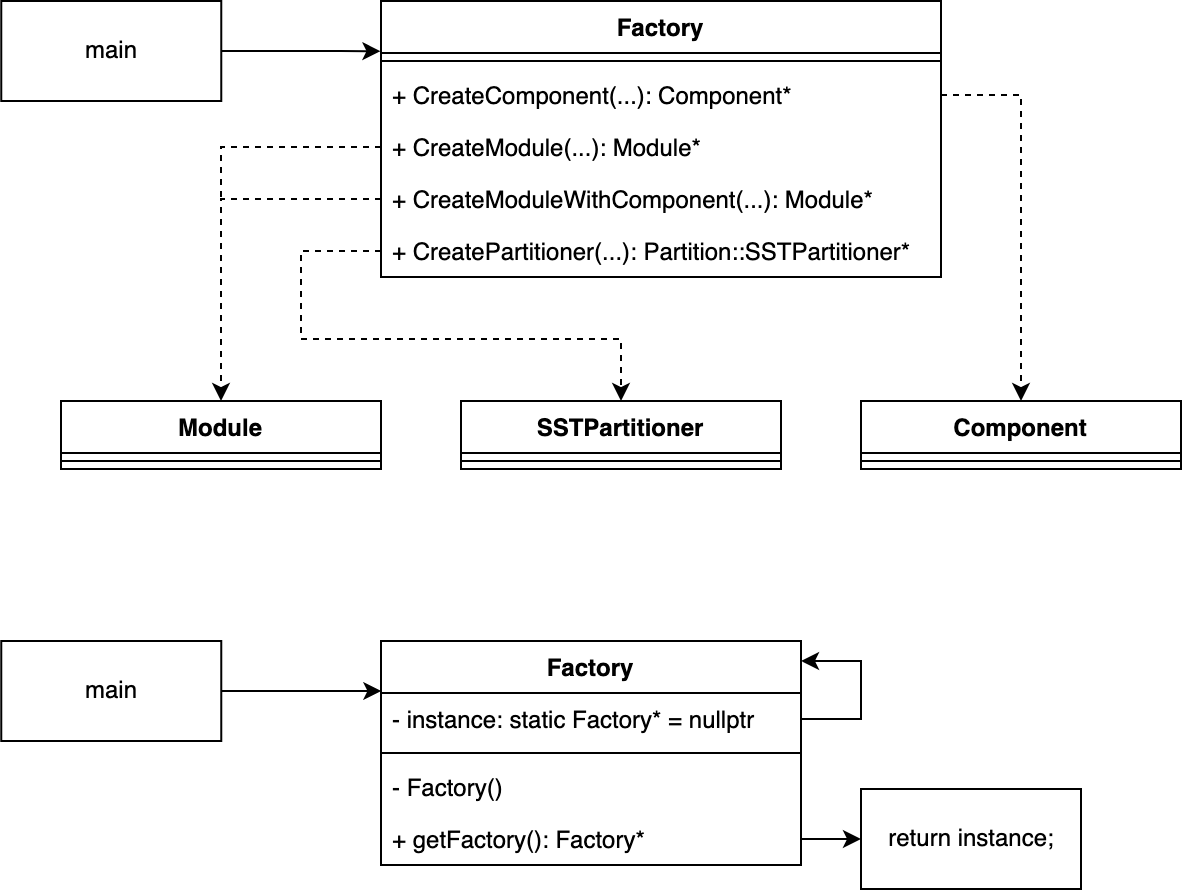
\includegraphics[width=0.8\textwidth]{af.png}
\end{figure}

Each of the methods accept parameters to instantiate the corresponding ConcreteProducts. There are several Client classes that call these methods, including \texttt{Simulation}, \texttt{BaseComponent} and the \texttt{main} function itself.



\subsection{Singleton Pattern}
The singleton pattern is present in the \texttt{Factory} and \texttt{Simulation.Simulation\_impl} classes. In the repository, the classes can be located at \texttt{factory.h} and \texttt{Simulation\_impl.h} respectively.

\subsubsection{Factory}
The \texttt{Factory} class is used to instantiate other concrete simulation classes. SST requires objects to be synchronized throughout the kernel, especially since they can be running on a distributed system where race conditions can become major issues. The software forces these simulation objects to be Singletons.

\begin{figure}[ht]
  \caption{Factory Implementing the Singleton Pattern}
  \centering
  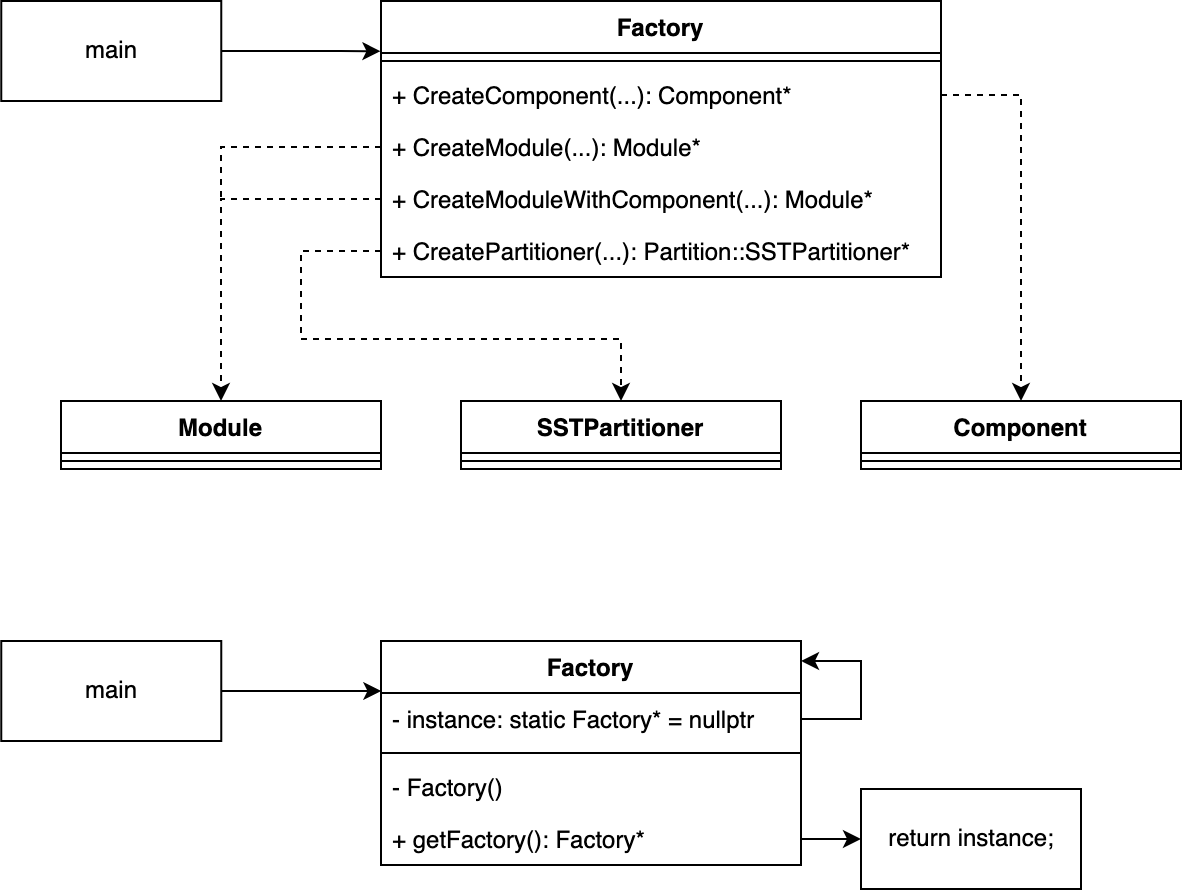
\includegraphics[width=0.8\textwidth]{singleton.png}
\end{figure}
\newpage

Listing \ref{singleton} demonstrates the \texttt{Factory} class following the typical steps dictated by the pattern.

\begin{lstlisting}[style=customC++,label=singleton,caption=Factory Implementing the Singleton Pattern \\ Files: src/sst/core/factory.h and src/sst/core/factory.cc]
class Factory {
  Factory(...);
  ~Factory();
  static Factory* instance;
}

Factory* Factory::instance = nullptr;

Factory::Factory(...) {
  if (instance) {
    ...
    // exit 1
  }
  instance = this;
}
\end{lstlisting}

Although SST is primarily intended for multi-threaded applications, the \texttt{Factory} Singleton class does not utilize any locks to account for the potential issues imposed by concurrency. Locks do exist in abundance throughout the project and within the class itself, but not when checking for instances of the class in other threads. The \texttt{Factory} class is responsible for creating SST Components, SubComponents, Modules, etc. as models for the simulation.

It appears that the Singleton is instantiated by \texttt{mpirun} as a single thread which spawns the other processes after it completes the analysis of the configuration options. The intent of the pattern is still preserved, although with the aforementioned assumptions that the executable instantiates it with a single thread.
\newpage

\subsubsection{Simulation\_impl}

\begin{figure}[ht]
  \caption{Simulation\_impl Implementing the Singleton Pattern}
  \centering
  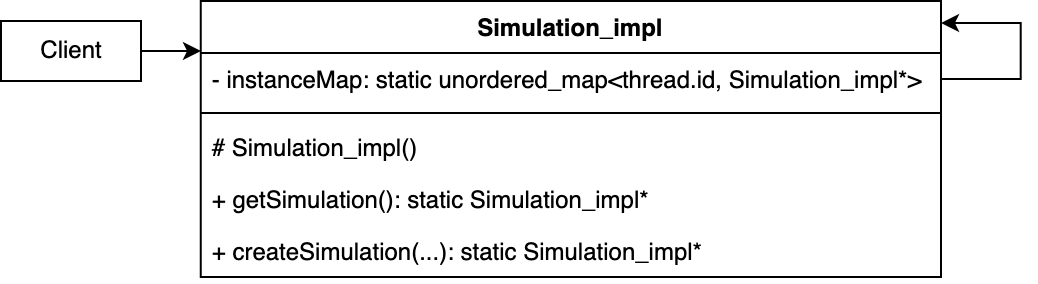
\includegraphics[width=0.8\textwidth]{singleton2.png}
\end{figure}

Listing \ref{simClassDecl} demonstrates the declaration of the other Singleton class, \texttt{Simulation\_impl}.

\begin{lstlisting}[style=customC++,label=simClassDecl,caption=Excerpt of Simulation\_impl Interface \\ File: src/sst/core/simulation\_impl.h]
class Simulation_impl : public Simulation {
public:
  static Simulation_impl* getSimulation();
  static Simulation_impl* createSimulation();
  static void shutdown();
protected:
  Simulation_impl(...) {}
private:
  static std::unordered_map<std::thread::id, Simulation_impl*> instanceMap;
}
\end{lstlisting}

Unlike \texttt{Factory}, this class is used by multiple classes in the framework which potentially may be on multiple threads. The \texttt{Simulation\_impl} class does implement a relatively safer version of a Singleton instance by using a mutex.

Listing \ref{singleton2} demonstrates the \texttt{Simulation\_impl} class following the typical steps dictated by the pattern, using a mutex to account for potential issues raised by multi-threaded processes.

\begin{lstlisting}[style=customC++,label=singleton2,caption=Simulation\_impl Implementing the Singleton Pattern \\ File: src/sst/core/simulation\_impl.cc]
std::unordered_map<std::thread::id, Simulation_impl*>
  Simulation_impl::instanceMap;

Simulation_impl* getSimulation() {
  return instanceMap.at(std::this_thread::get_id());
}

Simulation_Impl::createSimulation(...) {
  std::thread::id tid = std::this_thread::get_id();
  Simulation_impl* instance = new Simulation_impl(...);

  std::lock_guard<std::mutex> lock(simulationMutex);
  instanceMap[tid] = instance;
  ...
  return instance;
}

void Simulation_impl::shutdown() {
  instanceMap.clear();
}
\end{lstlisting}

\texttt{Simulation\_impl} appears to create an instance of itself on every thread and store them in the static unordered\_map attribute, instanceMap. Each of the instances follows the restrictions enacted by the Singleton pattern. This method allows for a Singleton object on every thread and therefore the core intent of the pattern remains preserved. The map's contents are destroyed with the public \texttt{shutdown} method which is accessible by the main function, which runs on the primary thread.


\subsection{Prototype Pattern}
The Prototype pattern is present in the project, although in a very limited manner. Select \texttt{SST.Core.Interfaces} classes implement a \texttt{clone} method to provide the ability to copy instances of themselves. The \texttt{StringEvent} class provides a shallow copy of itself to instantiate its ConcretePrototype, while \texttt{SimpleNetwork.Request} performs a deep copy.

\begin{figure}[h]
  \caption{SST Classes Implementing the Prototype Pattern}
  \centering
  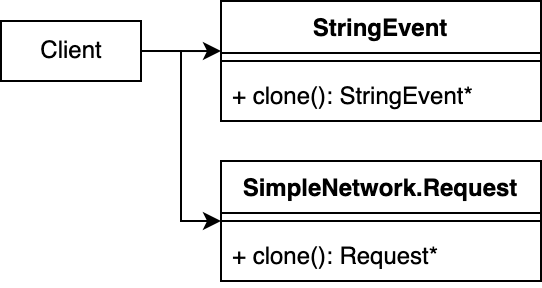
\includegraphics[width=0.8\textwidth]{proto.png}
\end{figure}

The following listings demonstrate the instances of the project following the typical steps dictated by the pattern:

\begin{lstlisting}[style=customC++,label=prototype1,caption=StringEvent Implementing the Prototype Pattern \\ File: src/sst/core/interfaces/stringEvent.h]
class StringEvent : public SST::Event, ... {
  virtual Event* clone() override {
    return new StringEvent(*this);
  }
}
\end{lstlisting}

\begin{lstlisting}[style=customC++,label=prototype2,caption=SimpleNetwork::Request Implementing the Prototype Pattern \\ File: src/sst/core/interfaces/simpleNetwork.h]
class SimpleNetwork : public SubComponent {
  class Request : public ... {
    Request* clone() {
      Request* req = new Request(*this);
      if (payload != nullptr) {
        req->payload = payload->clone();
      }
      return req;
    }
  }
}
\end{lstlisting}

\section{Recommended Software Patterns in SST}
The following patterns can be considered appropriate to implement in the project:
\begin{enumerate}
  \item Façade pattern
  \item Interpreter pattern
\end{enumerate}

\subsection{Façade Pattern}
The current method for a Client to interface the library is to create a derived class of Component and override its methods. While this approach provides extensive control over the functionality of crucial methods such as \texttt{void setup(unsigned int)}, \texttt{void finish(unsigned int)} and \texttt{bool tick(SST::Cycle\_t)}, it requires the Client to have extensive knowledge of the subsystems in the framework. The aforementioned methods, if overridden by the Client, must be implemented properly for the model and the simulation to be functional.

Listing \ref{currentModel} is an interface of a simple Component that simulates a primitive full adder hardware unit.

\begin{figure}[h]
  \caption{Circuit Design of a Simple Full Adder}
  \centering
  
\includegraphics[width=0.6\textwidth]{circuit.png}
\end{figure}

\newpage
\begin{lstlisting}[style=customC++,label=currentModel,caption=Example Interface of an SST Component Model]
#include <sst/core/component.h>
#include <sst/core/interfaces/stringEvent.h>
#include <sst/core/link.h>

class FullAdder : public SST::Component {
public:
  // register and manually configure each of the SST::Links
  // to their corresponding event handlers
  FullAdder(SST::ComponentId_t id, SST::Params& params);

  // implement logic for the model when it is being loaded into
  // the simulation
  void setup() override;

  // implement logic for the model when it is being unloaded from
  // the simulation
  void finish() override;

  // implement logic for the model on every clock cycle in the
  // simulation
  bool tick(SST::Cycle_t cycle);

  // event handlers for all the member SST::Link attributes
  void handle_A(SST::Event* event);
  void handle_B(SST::Event* event);
  void handle_C_in(SST::Event* event);

  // register the component
  SST_ELI_REGISTER_COMPONENT(
    FullAdder, // class
    "fulladder", // element library
    "fulladder", // component
    SST_ELI_ELEMENT_VERSION(1, 0, 0),
    "SST example model",
    COMPONENT_CATEGORY_UNCATEGORIZED)

  // port name, description, event type
  SST_ELI_DOCUMENT_PORTS(
    {"A", "Operand 1", {"sst.Interfaces.StringEvent"}},
    {"B", "Operand 2", {"sst.Interfaces.StringEvent"}},
    {"C_in", "Carry-in", {"sst.Interfaces.StringEvent"}},
    {"S", "Sum", {"sst.Interfaces.StringEvent"}},
    {"C_out", "Carry-out", {"sst.Interfaces.StringEvent"}})

private:
  std::string clock;  // SST parameters
  // SST links
  SST::Link *A_link, *B_link, *C_in_link, *S_link, *C_out_link;
  // other attributes
  std::string A, B, C_in;
  SST::Output output;
};
\end{lstlisting}
\newpage

This Component is a relatively simple example of a model that can be simulated in the SST framework. The hardware logic for the full adder will be implemented in the tick function, where the output values (\texttt{S} and \texttt{C\_out}) are evaluated using the member attributes \texttt{A}, \texttt{B}, and \texttt{C\_in} after they are processed by their corresponding handlers.

Exposing all the complexity of the base methods to the Client can lead to many potential issues. One way to reduce the chances of such issues is to abstract away the steps and methods from the Client using a Facade design pattern. The library, in its current state, does not provide a method to call any of the constructors of the Simulation objects, such as Components and SubComponents. Execution of such objects is done through various command line tools. Even testing of the classes appear to be done through external tools and Python interpreters, which compare the outputs to the expected outputs rather than using asserts.

The following listing is a potential interface that may be possible with the integration of a Facade object into the project.

\begin{lstlisting}[style=customC++,label=facade,caption=Potential Implementation of Facade]
SST::Facade* facade = new SST::Facade(argc, argv);
SST::Component* component = facade->getComponent();

component->register(
  "FullAdder", // class name
  "fulladder", // element library
  "fulladder", // component
  "1.0.0",
  "SST parent model");
component->registerStringEventPort("A", "Operand 1");
...

component->overrideTick(&customTickFunc);
component->setMPIRank(0);
component->run();

delete component;
delete facade;
\end{lstlisting}

\newpage
\subsection{Interpreter Pattern}
SST requires external Python scripts to configure and run the Client models. The configuration file provides a vast amount of options; from setting the duration of the simulation to providing custom parameters to the models. The configuration file is imported by the provided executables and parsed by the \texttt{Model::Python} classes. The classes map the parameterized method calls made in the configuration file to the implemented class methods.

This method of interpreting the configuration file to generate SST Components for its simulation requires the usage of a Python interpreter. This external dependency potentially adds unnecessary overhead that can be circumvented by integrating the Interpreter pattern into the project. Adding an AbstractExpression class in native C++ will allow the project to not have to rely on an external framework and language to run its simulations.

Instead of a Python script, the simulation configuration can be represented in an XML format. XML parsing is a fairly common task in commercial software that is often achieved by external libraries. Configuration options in SST may require a very simple parser. The AbstractExpression class will perform a similar role to the current \texttt{Model::Python} classes and create SST Components for the simulation.

The following listing is an example of a configuration file for the preceding FullAdder model.
\begin{lstlisting}[style=customPython,label=runPy,caption=Example SST Configuration File \\ File: run.py]
import sst

sst.setProgramOption("stopAtCycle", "5s")

full_add_0 = sst.Component("Full Adder 0", "fulladder.fulladder")
full_add_0.addParams({"clock": "1Hz"})

full_add_1 = sst.Component("Full Adder 1", "fulladder.fulladder")
full_add_1.addParams({"clock": "1Hz"})

full_add_2 = sst.Component("Full Adder 2", "fulladder.fulladder")
full_add_2.addParams({"clock": "1Hz"})

full_add_3 = sst.Component("Full Adder 3", "fulladder.fulladder")
full_add_3.addParams({"clock": "1Hz"})

sst.Link("C_out0").connect(
    (full_add_0, "C_out0", "1ps"),
    (full_add_1, "C_in1", "1ps")
)
sst.Link("C_out1").connect(
    (full_add_1, "C_out1", "1ps"),
    (full_add_2, "C_in2", "1ps")
)
sst.Link("C_out2").connect(
    (full_add_2, "C_out2", "1ps"),
    (full_add_3, "C_in3", "1ps")
)
\end{lstlisting}

The following listing is a potential translation of the preceding configuration file.
\begin{lstlisting}[style=customXML,label=xml,caption=Potential Implementation of an SST Configuration File \\ File: run.xml]
<? xml version="1.0" encoding="UTF-8"?>
<config>
  <setProgramOption stopAtCycle="5s"/><setProgramOption/>
  <component id="full_add_0" name="Full Adder 0" class="fulladder"/>
    <param key="clock" value="1Hz"/><param/>
    <link from="C_out0" to="full_add_1" port="C_in1"/></link>
  <component/>
  <component id="full_add_1" name="Full Adder 1" class="fulladder"/>
    <param key="clock" value="1Hz"/><param/>
    <link from="C_out1" to="full_add_2" port="C_in2"/></link>
  <component/>
  <component id="full_add_2" name="Full Adder 2" class="fulladder"/>
    <param key="clock" value="1Hz"/><param/>
    <link from="C_out2" to="full_add_3" port="C_in3"/></link>
  <component/>
  <component id="full_add_3" name="Full Adder 3" class="fulladder"/>
    <param key="clock" value="1Hz"/><param/>
  <component/>
</config>
\end{lstlisting}

\subsection{Other Minor Idioms}
The project can be found with several \texttt{goto} statements within the code base. The use of this unconditional jump is highly discouraged in the C++ community, although its usage is not considered a part of any idioms. Regardless, the project would benefit from discarding these statements and replacing them with proper conditional jumps for increased clarity and understanding of the project.

\begin{appendices}
    \section{Full Adder Hardware Design}
    The contents...
\end{appendices}

\bibliographystyle{plain}
\bibliography{ref}

\end{document}
